% !TEX root = main.tex

\newchapter{Finite Differenzen Methode}{}
\newsection{Theoretische Grundlagen}{}
Das zu lösende Randwertproblem ist wie folg definiert:
\begin{align}
	\label{eq:Randwretproblem}
	-\varepsilon \Delta V &=  \rho  \text{ mit }\\
	V &= V_D \text{ auf } \Gamma_D \nonumber\\
	\pDiff{V}{n} &= V_N \text{ auf } \Gamma_N \nonumber
\end{align}

wobei \begin{align}
	\label{eq:LaplaceV}
	\Delta V = \pDiffDiff{V}{x} + \pDiffDiff{V}{y} + \pDiffDiff{V}{z}
\end{align}

In den gegebenen Beispielen ist $\varepsilon$ konstant und $\neq 0$, $\rho = 0$ und $V_N = 0$. Des Weiteren gilt aufgrung der Ausdehnung des Problems $\pDiff{}{z} = 0$, womit sich das Randwertproblem (\ref{eq:Randwretproblem}) wie folgt vereinfacht:
\begin{align}
	\label{eq:Randwertproblem_simple}
	&\pDiffDiff{V}{x} + \pDiffDiff{V}{y} = 0 \text{ mit }\\
	&V = V_D \text{ auf } \Gamma_D \nonumber\\
	&\pDiff{V}{n} = 0 \text{ auf } \Gamma_N \nonumber
\end{align}

Man nehme nun eine konstante \textit{Schrittweite} $h$ an und führe folgende Notation ein:
\begin{align*}
	V_{i,j} = V(ih,jh),\quad i,j\geq 0
\end{align*}

Die Linearisierung der Differentialgleichung in \myRef{eq:Randwertproblem_simple} liefert somit
\begin{align*}
	\frac{V_{i+1,j} - 2V_{i,j} + V_{i-1,j}}{h^2} + \frac{V_{i,j+1} - 2V_{i,j} + V_{i,j-1}}{h^2} = 0
\end{align*}
bzw. unter Berücksichtigung der Konstanz von $h$
\begin{align}
	\label{eq:lin_eq}
	-4V_{i,j} + V_{i+1,j} + V_{i-1,j} + V_{i,j+1} + V_{i,j-1} = 0.
\end{align}

Das Problemgebiet wird somit in Quadrate der Seitenlänge $h$ diskretisiert wobei die \textit{Knotenpotentiale} an den Gitterknotenpunkten durch Lösen des aus \myRef{eq:lin_eq} entstehenden linearen Gleichungssystems ermittelt werden. Die vorgegebenen Potentiale am dirichletschen Rand $\Gamma_D$ fließen als bekannte Größen in das Gleichungssystem ein. \newline
Ferner sei ohne weitere Herleitung gesagt, dass die Behandlung der \textbf{homogenen} neumannschen Randbedingungen keiner weiteren Aufmerksamkeit bedarf. Hier sei auf die entsprechende Fachliteratur verwiesen. \newline
Die genaue Vorgehensweise zur Lösung des Problems mit der oben genannten Methode wird im folgenden Kapitel anhand eines einfachen Beispiels erläutert.

 \newsection{Funktion des FDM-Algorithmus}{}
 Abbildung 1 zeigt ein Problem äquivalent jenem aus Beispiel 1 der Hausübung, allerdings mit weitaus geringerer Auflösung.
 \begin{figure}[htbp]
 	\centering
 	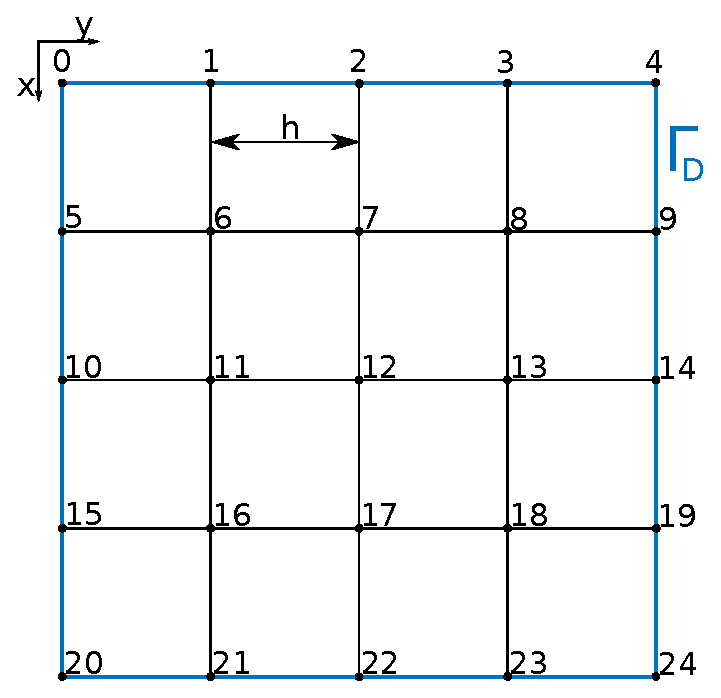
\includegraphics[scale=1]{pics/grid_1.eps}
 	\caption{Problemgebiet}
 	\label{fig:grid_1}
 \end{figure}
	
	In einem ersten Schritt wird jedem Knoten eine eindeutige Nummer $n$  zugewiesen welche mittels einer Tabelle den Positionsindizes $i$ und $j$ zugewiesen wird:\newline
	
\begin{table}[htbp]
	\centering
\begin{tabular}{c|c|c}
$\mathbf{i}$	& $\mathbf{j}$ & $\mathbf{n}$ \\
	\hline\hline
	0&0&0\\
	0&1&1\\
	0&2&2\\
	.&&\\
	.&&\\
	.&&\\
	4&4&24
\end{tabular}
\caption{Zuordnung der Knotennummer zu den Koordinatenindizes}
\end{table}
Im Weiteren sei $N_{Knoten}$ die Gesamtanzahl der Knoten.
     
In einem weiteren Schritt werden zwei weitere Tabellen erstellt von denen die Erste die Knoten am dirichletschen Rand $\Gamma_D$ und die entsprechenden Knotenpotentiale enthält. Im Weiteren sei $N_D$ die Anzahl der Knoten auf $\Gamma_D$.\newline
\begin{table}[htbp]
	\centering
\begin{tabular}{c|c}
	$\mathbf{n}$	&$\mathbf{V}$ \\
	\hline\hline
	0 & 100\\
	2 & 100\\
	.&\\
	.&\\
	.&\\
\end{tabular}
\caption{Zuordnung der Randknoten zu den entsprechenden Randwerten}
\end{table}



Das zu Problem und somit auch das zu lösende Gleichungssystem besitzt nun somit $N_{Unbek} = N_{Knoten}-N_D$.\newline

$\m{A}$ sei die $\left(N_{Unbek}\times N_{Unbek}\right)$-Matrix mit den aus \myRef{eq:lin_eq} berechneten Koeffizienten.
Weiters sei $\m{x}$ der $\left(N_{Unbek}\times 1\right)$-Vektor der unbekannten Knotenpotentiale sowie $\m{b}$ der $\left(N_{Unbek}\times 1\right)$-Vektor der bekannten Werte.\newline

Das zu lösende Gleichungssystem lautet somit
\begin{align}
	\label{eq:eq_sys}
	\m{A}\m{x}=\m{b}.
\end{align}

Die oben erwähnte zweite Tabelle ordnet die Knotennummern der unbekannten Knotenpotentiale ihrer Position im Gleichungssystem zu. So stellt zum Beispiel der Knoten 6 das erste Unbekannte Element im Gleichungssystem dar. Der Knoten 7 das Zweite usw. 

\begin{table}[htbp]
	\centering
	\begin{tabular}{c|c}
		$\mathbf{n}$	&Position in $\m{x}$ \\
		\hline\hline
		6&1\\
		7&2\\
		8&3\\
		11&4\\
		12&5\\
		.&\\
		.&\\
		.&\\
	\end{tabular}
	\caption{Zuordnung der unbekannten Knotenpotentiale zu ihrer Position in $\m{x}$}
\end{table}

Im nächsten Schritt wird das Gleichungssystem \myRef{eq:eq_sys} durch iteratives Anwenden von \myRef{eq:lin_eq} über alle unbekannten Knoten assembliert. Die Iteration erfolgt dabei nach steigender Knotennummer.\newline
Abbildung \ref{fig:grid_2} zeigt exemplarisch die Vorgehensweise für Knoten 6.

\begin{figure}[htbp]
	\centering
	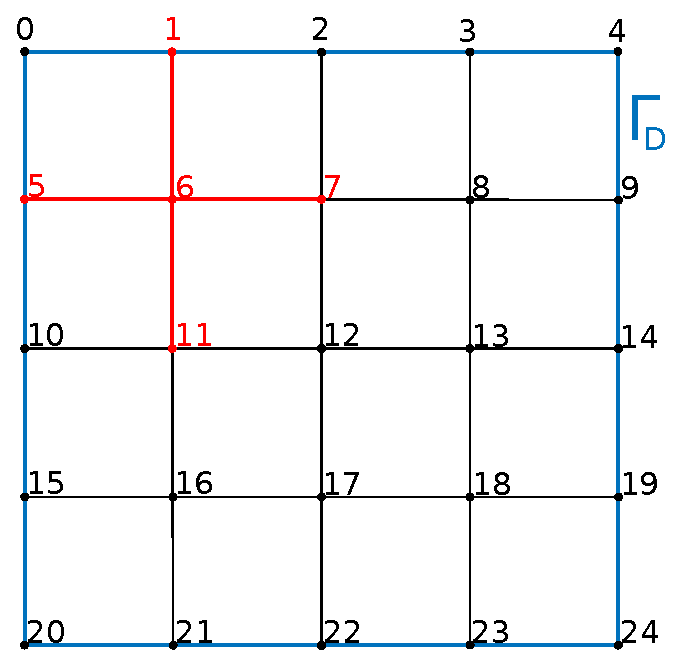
\includegraphics[scale=1]{pics/grid_2.eps}
	\caption{FDM-'Stern' für Knoten 6}
	\label{fig:grid_2}
\end{figure}

Die entsprechende Gleichung des Gleichungssystems lautet
\begin{align*}
	-4V_{1,1} + V_{2,1} + V_{0,1} + V_{1,2} + V_{1,0} = 0,
\end{align*} wobei 
\begin{itemize}
\item $V_{1,1} = V_6$, unbekannt,
\item $V_{2,1} = V_{11}$, unbekannt,
\item $V_{0,1} = V_1$, bekannt,
\item $V_{1,2} = V_7$, unbekannt und
\item $V_{1,0} = V_5$, bekannt
\end{itemize}
gilt.
Somit lautet die erste Gleichung des Gleichungssystems
\begin{align}
	-4V_{1,1} + V_{2,1} + V_{1,2} = -V_{0,1} - V_{1,0}.
\end{align}

Analog dazu kann für alle weiteren Knoten vorgegangen werden. Das Ergebnis ist eine symmetrische und quadratische Matrix $\m{A}$. Das Lösen besagten Gleichungssystems liefert die unbekannten Knotenpotentiale.

 \newsection{Weiterverarbeitung der Lösung}{}
 Aus der im vorherigen Kapitel ermittelten Lösung für die Knotenpotentiale soll nun in einem letzten Schritt das elektrische Feld bzw. das stationäre Strömungsfeld berechnet werden.\newline
 
 Die Linearisierung des Zusammenhangs
 \begin{align*}
 	\m{E} = -\nabla V = 	
 	\begin{bmatrix}
 		\pDiff{V}{x}\\
 		\pDiff{V}{y}\\
 		\pDiff{V}{z}
 	\end{bmatrix} 
 \end{align*}
liefert mit $\pDiff{V}{z}$
\begin{align}
	\m{E}\approx \begin{bmatrix}
	\frac{V_{i+1,j} - V_{i,j}}{h}\\
	\frac{V_{i+1,j} - V_{i,j}}{h}
	\end{bmatrix} 
\end{align}

Die Berechnung des elektrischen Feldes an den Knotenpunkten erfolgt 'links oben' im Problemgebiet bei $i = 0$ und $j = 0$ und wirt iterativ fortgesetzt, wobei zu beachten ist dass am rechten und unteren Rand keine Feldberechnung durchgeführt werden kann da dort die Indizes $i+1$ und $j+1$ aus dem Problemgebiet herausragen.\newline


\newchapter{Aufgabe 1}{}
\newsection{Numerische Berechnung}{}
Gewählte Diskretisierung: $\frac{L}{100}$\newline

\textbf{Diskussion der Ergebnisse:}
Durch die bündig anschließenden Flächen des dirichletschen Randes kommt es zu Singularitäten der Magnitude des elektrischen Feldes in den Ecken des Problemgebiets. Siehe hierzu die Abbildungen \ref{fig:mag_E_1}, \ref{fig:mag_E_2} und \ref{fig:mag_E_3}
\newsubsection{Fall a)}{}

\begin{figure}[H]
	\centering
	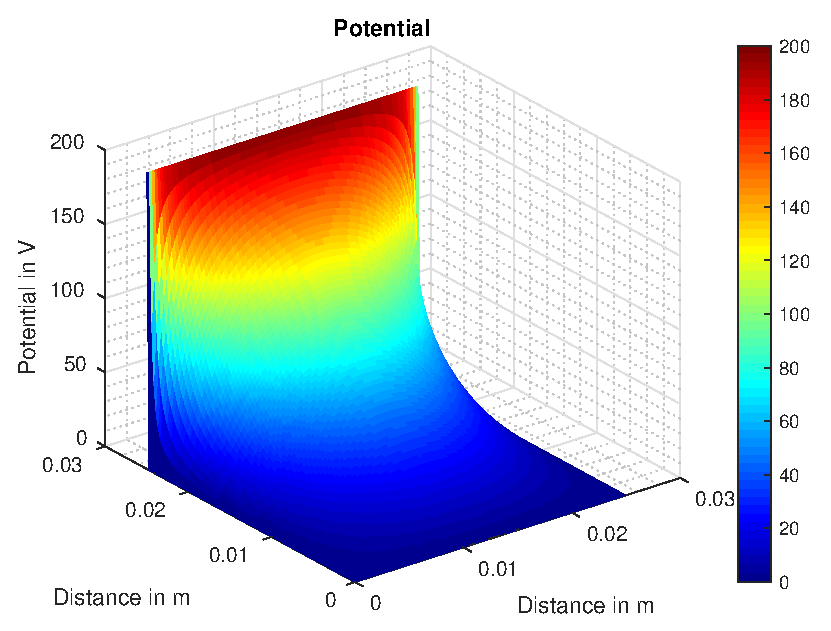
\includegraphics[scale=1]{pics/Bsp_1_a/fig_1.eps}
	\caption{Potentialverlauf}
\end{figure}

\begin{figure}[H]
	\centering
	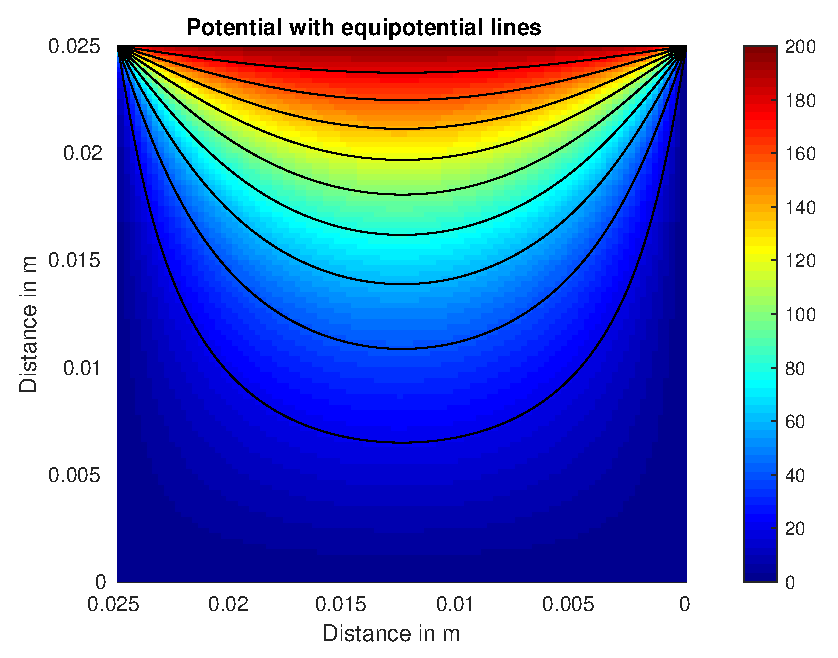
\includegraphics[scale=1]{pics/Bsp_1_a/fig_2.eps}
	\caption{Potentialverlauf mit Equipotentiallinien}
\end{figure}

\begin{figure}[H]
	\centering
	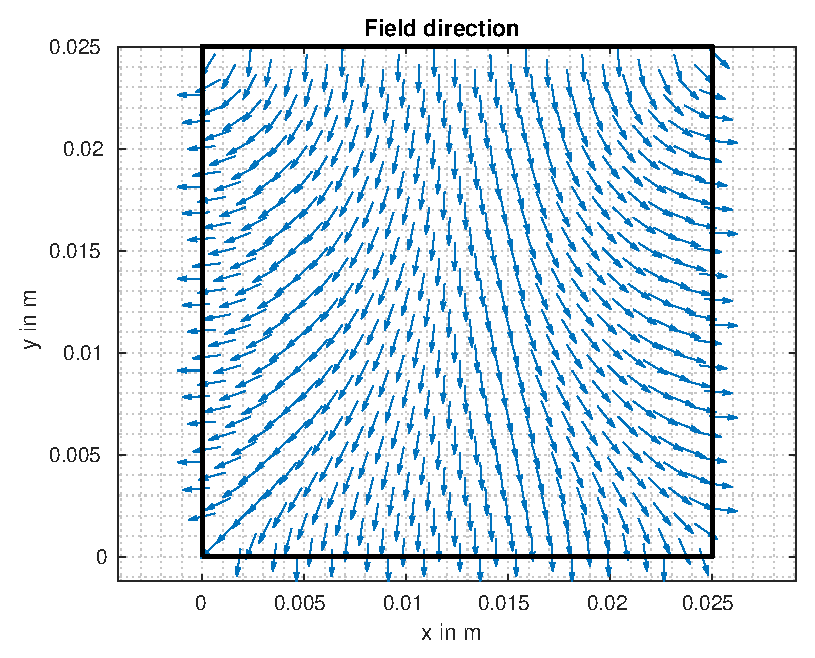
\includegraphics[scale=1]{pics/Bsp_1_a/fig_3.eps}
	\caption{Richtung des elektrischen Feldes}
\end{figure}

\begin{figure}[H]
	\centering
	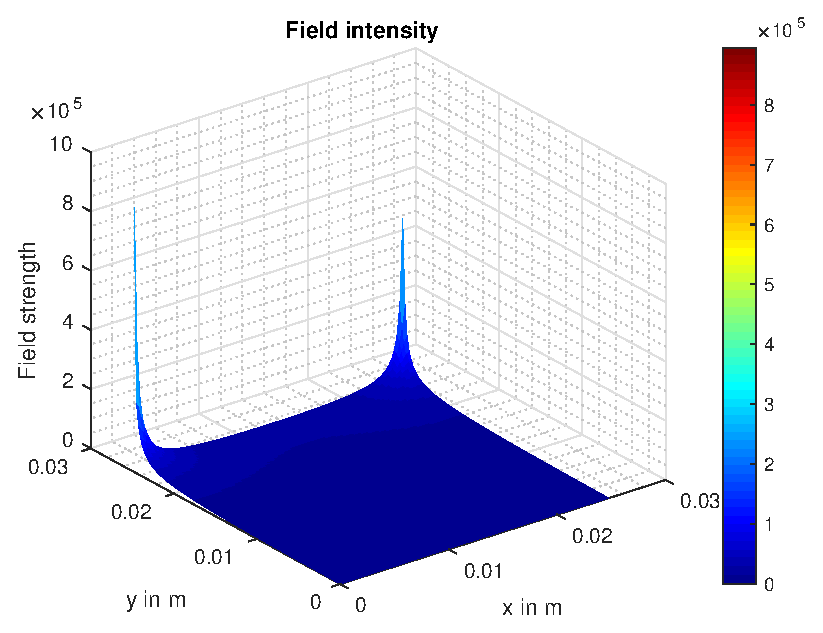
\includegraphics[scale=1]{pics/Bsp_1_a/fig_4.eps}
	\caption{Magnitude des elektrischen Feldes}
	\label{fig:mag_E_1}
\end{figure}


\newsubsection{Fall b)}{}

\begin{figure}[H]
	\centering
	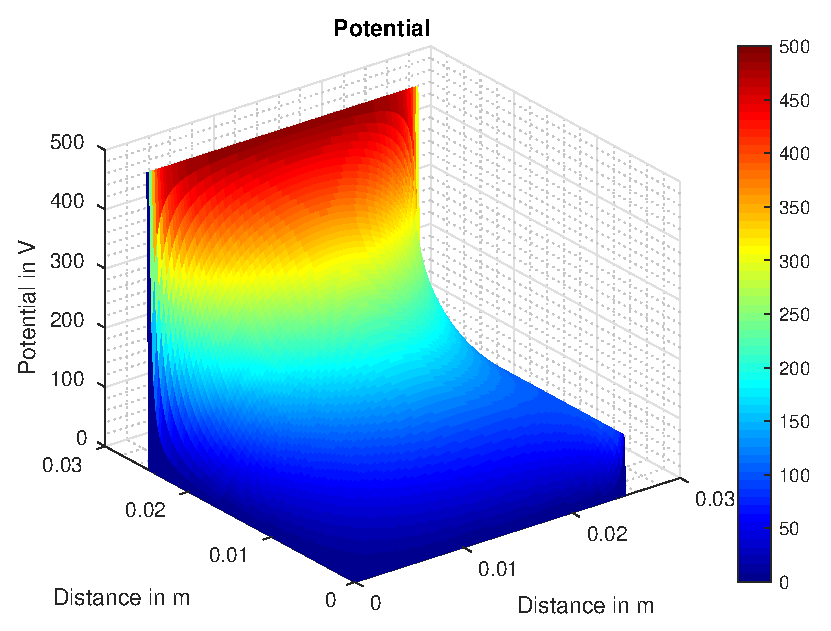
\includegraphics[scale=1]{pics/Bsp_1_b/fig_1.eps}
	\caption{Potentialverlauf}
\end{figure}

\begin{figure}[H]
	\centering
	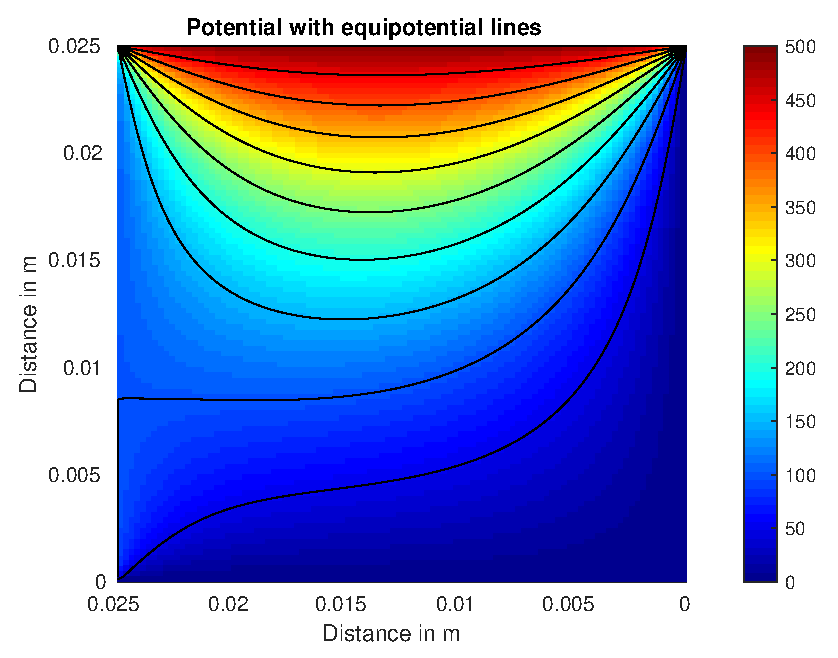
\includegraphics[scale=1]{pics/Bsp_1_b/fig_2.eps}
	\caption{Potentialverlauf mit Equipotentiallinien}
\end{figure}

\begin{figure}[H]
	\centering
	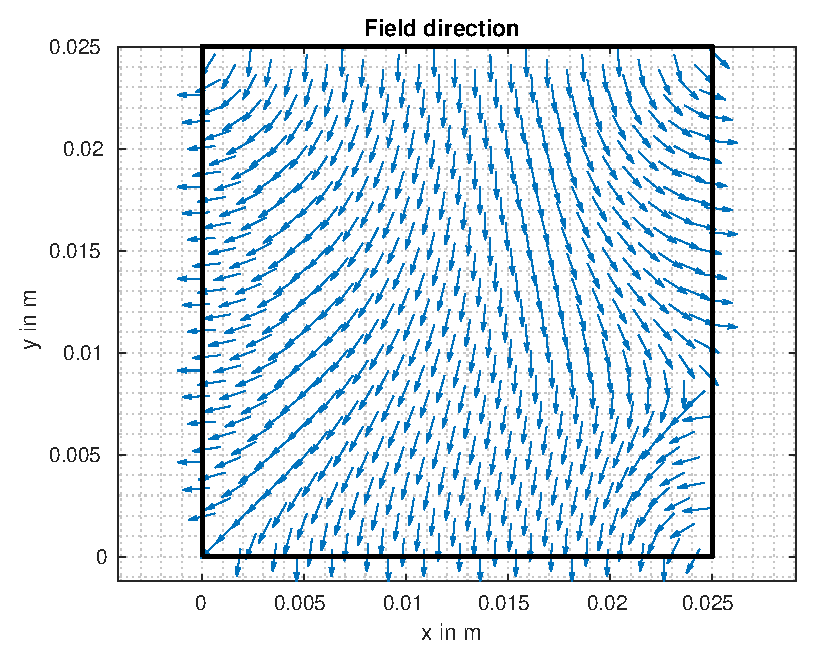
\includegraphics[scale=1]{pics/Bsp_1_b/fig_3.eps}
	\caption{Richtung des elektrischen Feldes}
\end{figure}

\begin{figure}[H]
	\centering
	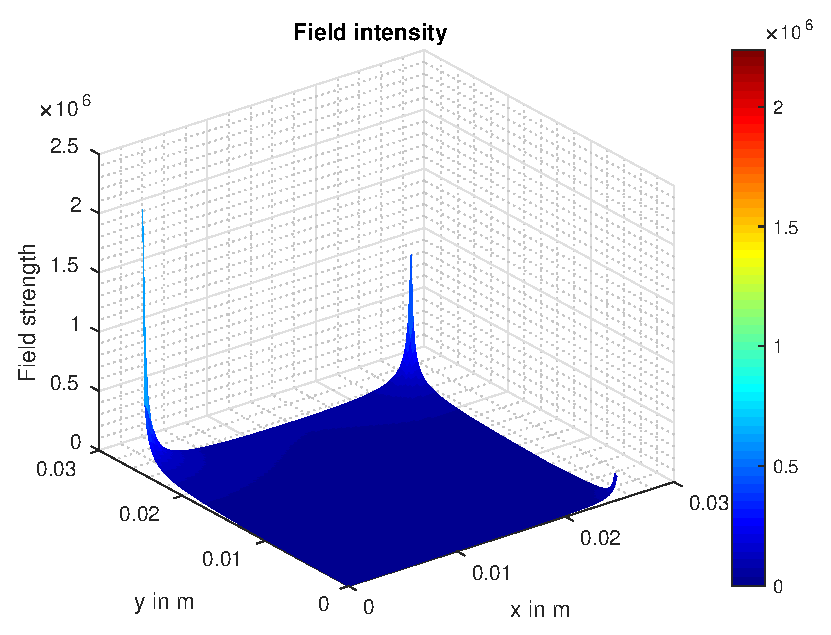
\includegraphics[scale=1]{pics/Bsp_1_b/fig_4.eps}
	\caption{Magnitude des elektrischen Feldes}
	\label{fig:mag_E_2}
\end{figure}

\newsubsection{Fall c)}{}

\begin{figure}[H]
	\centering
	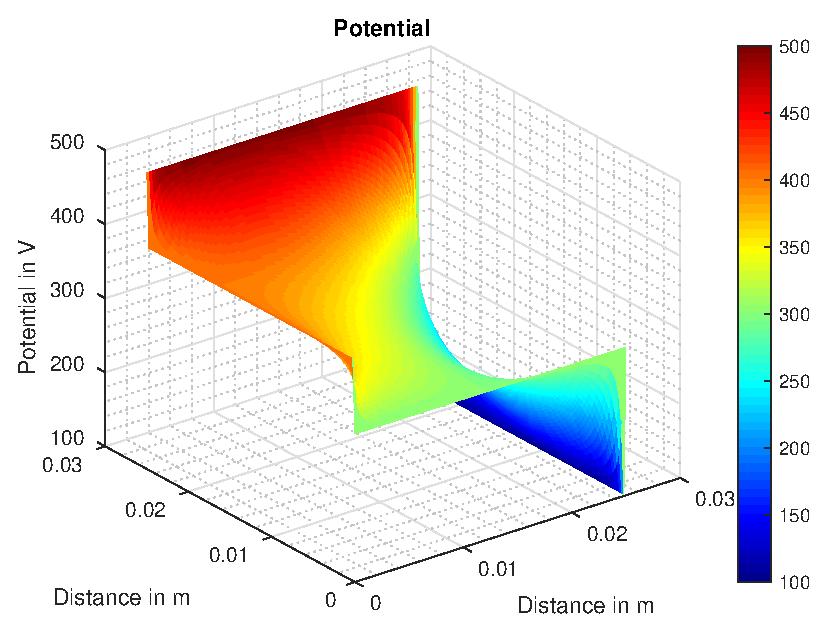
\includegraphics[scale=1]{pics/Bsp_1_c/fig_1.eps}
	\caption{Potentialverlauf}
\end{figure}

\begin{figure}[H]
	\centering
	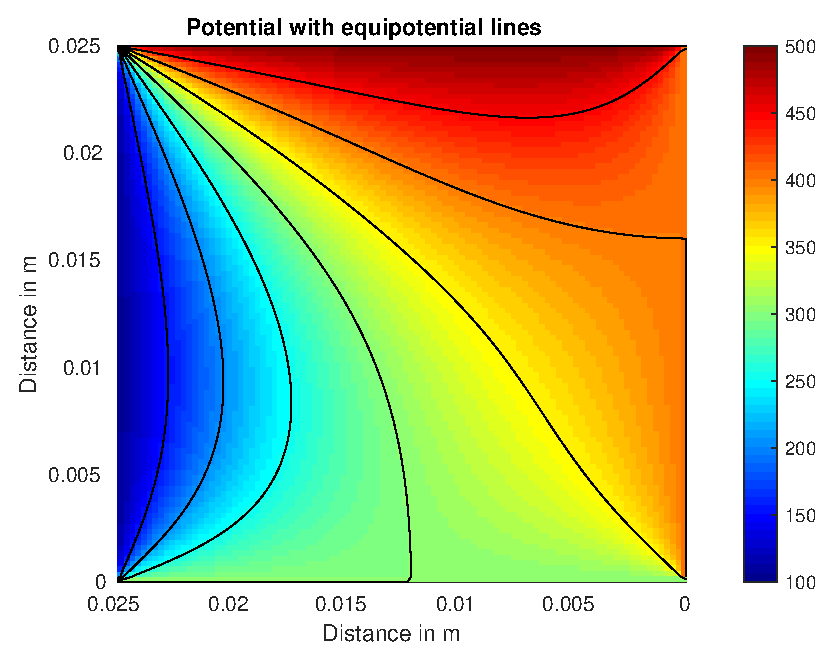
\includegraphics[scale=1]{pics/Bsp_1_c/fig_2.eps}
	\caption{Potentialverlauf mit Equipotentiallinien}
\end{figure}

\begin{figure}[H]
	\centering
	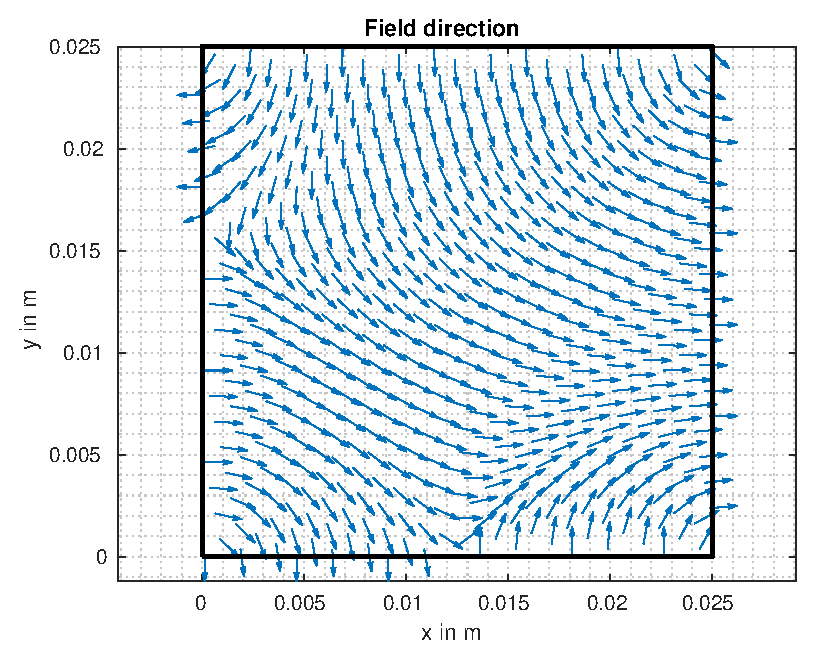
\includegraphics[scale=1]{pics/Bsp_1_c/fig_3.eps}
	\caption{Richtung des elektrischen Feldes}
\end{figure}

\begin{figure}[H]
	\centering
	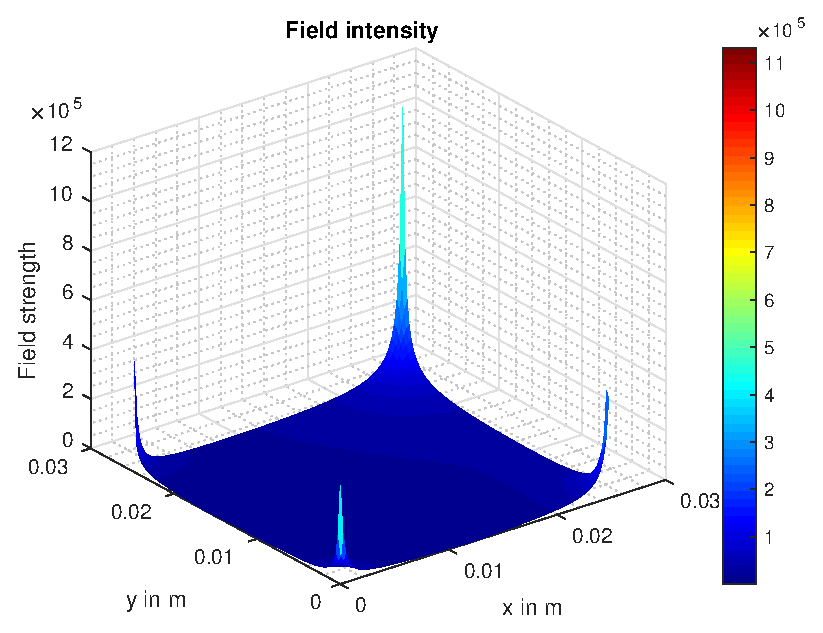
\includegraphics[scale=1]{pics/Bsp_1_c/fig_4.eps}
	\caption{Magnitude des elektrischen Feldes}
	\label{fig:mag_E_3}
\end{figure}

\newpage
\newsection{Aufgabe 2}{}

Gewählte Diskretisierung: $1\si{\milli\meter}$\newline

\textbf{Diskussion der Ergebnisse:}
Man beachte die Singularität der Magnitude des stationären Strömungsfeldes in Abbildung \ref{fig:mag_J}.

\begin{figure}[H]
	\centering
	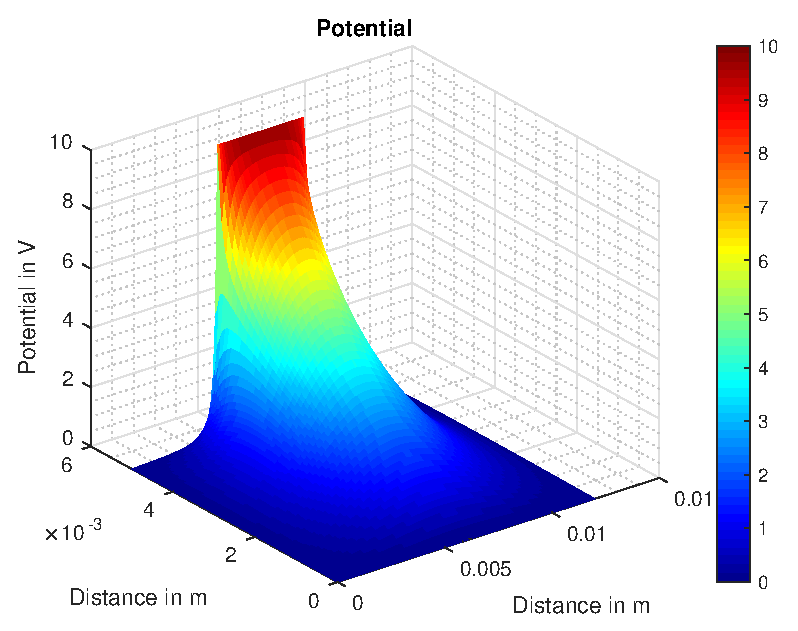
\includegraphics[scale=1]{pics/Bsp_2/fig_1.eps}
	\caption{Potentialverlauf}
\end{figure}

\begin{figure}[H]
	\centering
	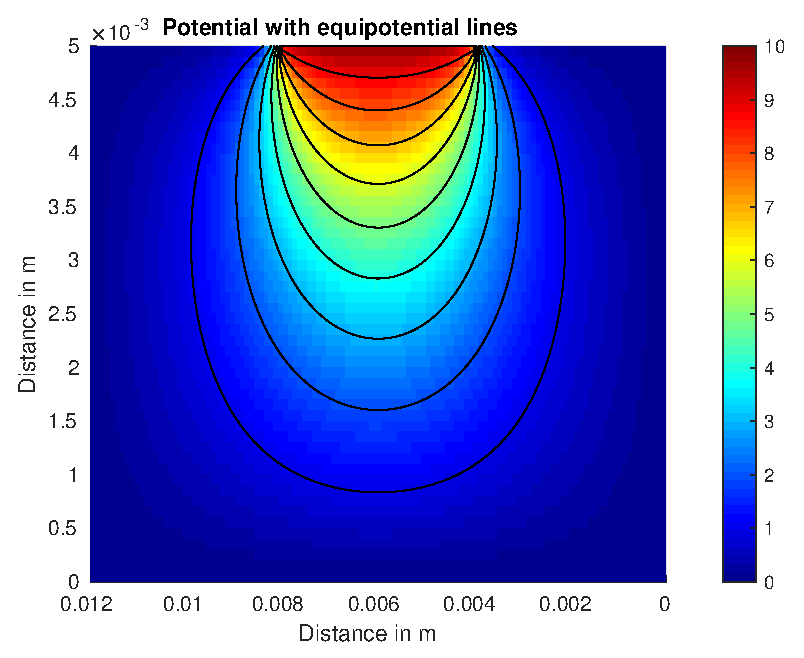
\includegraphics[scale=1]{pics/Bsp_2/fig_2.eps}
	\caption{Potentialverlauf mit Equipotentiallinien}
\end{figure}

\begin{figure}[H]
	\centering
	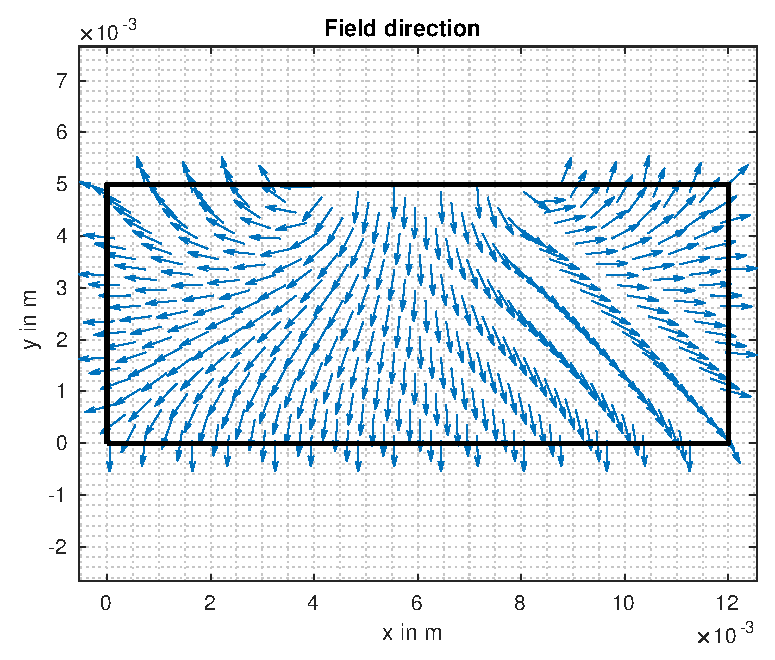
\includegraphics[scale=1]{pics/Bsp_2/fig_3.eps}
	\caption{Richtung des stationären Strömungsfeldes}
\end{figure}

\begin{figure}[H]
	\centering
	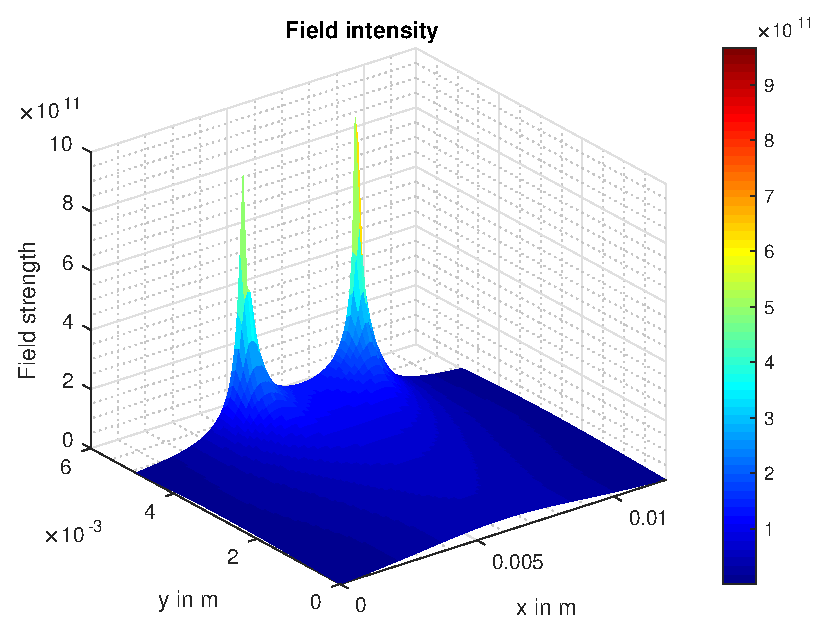
\includegraphics[scale=1]{pics/Bsp_2/fig_4.eps}
	\caption{Magnitude des stationären Strömungsfeldes}
	\label{fig:mag_J}
\end{figure}
